\documentclass[usegeometry=true]{scrartcl}
\usepackage[ngerman]{babel}
\usepackage[T1]{fontenc}
\usepackage{lmodern}
\usepackage[utf8]{inputenc}
\usepackage{hyperref}
\usepackage{amssymb}
\usepackage{graphicx}
% Dimensionen bitte nicht ändern. 
\usepackage[left=2cm, right=2cm, top=2cm, bottom=2cm, bindingoffset=1cm, includeheadfoot]{geometry}
%Zeilenabstand bitte nicht ändern
\usepackage[onehalfspacing]{setspace}
\usepackage[numbers]{natbib}
%\usepackage[backend=biber,style=numeric,]{biblatex}\addbibresource{literatur.bib}
\bibliographystyle{unsrtnat}


\begin{document}
% ----------------------------------------------------------------------------
\subject{Projektbericht zum Modul Information Retrieval und Visualisierung Sommersemester 2021}

\title{Bike Buyers 1000}
\subtitle{Visualisierung von Fahrradkaufdaten}
\author{Floyd Spuhler\\ Matrikelnummer: 216235360 \\ \href{https://github.com/floeagle/Bike-Buyers-1000}{Github-Repository}}

% obligatorisch


\date{10.09.2021}
\maketitle% verwendet die zuvor gemachte Angaben zur Gestaltung eines Titels
\thispagestyle{empty}
% ----------------------------------------------------------------------------
% Inhaltsverzeichnis:
\newpage
\thispagestyle{empty}
\tableofcontents
% ----------------------------------------------------------------------------
% Gliederung und Text:
\newpage
\pagenumbering{arabic}
\section{Einleitung}
Durch das wachsende Umweltbewusstsein in der Bevölkerung rückt besonders das Fahrrad als klimaneutrales Verkehrsmittel in den Fokus \cite{Marquart.2021}. Bereits 2019 betrug der Gesamtbestand an Fahrrädern in Deutschland fast 76 Millionen \cite{Kords.26.06.2020,Statista.25.08.2021}. Die anhaltende Covid-19 Krise verstärkt den zunehmenden Fahrrad-Boom für die Freizeitgestaltung und den Pendelverkehr \cite{Platter.2020}. Gründe hierfür liegen beispielsweise bei der Sportmöglichkeit als Ausgleich zu geschlossenen Sportstätten, sowie im Individualverkehr für das Einhalten der Abstandregeln als Alternative zum Nahverkehr. Dabei wird sich häufig für das Fahrrad anstelle des Autos entschieden \cite{Kollner.30.12.2020,Thomannbusse.24.11.2020}. Passend dazu gaben im Rahmen einer Studie 61\%  von 782 Fahrradfahrenden an, dass Sie während der Covid-19 Krise bei Kurzstrecken auf das Fahrrad zurückgreifen, weswegen auch die Nachfrage nach dem Ausbau von Fahrradstrecken steigt \cite{sinus.2021}. Um die Sicherheit von Fahrradfahrenden im Straßenverkehr zu verbessern, nimmt die Planung und der Bau neuer Fahrradstrecken in deutschen Städten zu \cite{sinus.2021,ADAC.05.09.2021,Muenchen.de.05.09.2021}. Durch die Krise bedingte Lieferverzögerungen und Knappheiten führen zu einer hohen Nachfrage und steigenden Preisen. Auch wärmere Winter begünstigen eine längere Fahrradsaison und sorgen dadurch zusätzlich für Lieferengpässe \cite{tagesschau.11.03.2021}. Gleichzeitig werden Neuentwicklungen, wie E-Bikes, immer beliebter, was sich an der Gesamtabsatzbeteiligung im Jahr 2020 von 38,7\% in Deutschland bemerkbar macht \cite{tagesschau.11.03.2021}. 
In der Schweiz ist das Fahrrad nicht zuletzt durch den staatlich geförderten Ausbau von Fahrradspuren zum beliebtesten Verkehrsmittel geworden \cite{Platter.2020}.

Lieferengpässe erschweren die Kapazitätsplanung und damit die Kundenbeziehung. Eine weitere Herausforderung ist der beschriebene Ausbau von Fahrradstrecken und die damit verbundene Planung. Daraus lassen sich die folgenden Fragen ableiten:
\begin{itemize}
\item Gibt es Auffälligkeiten bei der Visualisierung der Fahrraddaten, die zum Kauf führen? Gibt es hierbei Zusammenhänge?
\item Welche Anpassungen sind durch den Fahrrad-Boom in Bezug auf die Infrastruktur vorzunehmen?
\end{itemize}
Das Ziel dieser Arbeit ist es, diese Fragestellungen  aufzugreifen und mit Hilfe von Visualisierungstechniken, wie dem Scatterplot, Parallelen Koordinaten und dem Baumdiagramm zu beantworten. Durch diese Darstellungen können Zusammenhänge hervorgehoben werden und Kernaussagen entnommen werden. Durch die Interaktionsmöglichkeiten mit den Modellen können eigene Erkenntnisse oder Trends gewonnen und individuell hervorgehoben werden.    

\subsection{Anwendungshintergrund}


Diese Forschungsarbeit bereitet Informationen auf, die interessante Einblicke in das Kaufverhalten von Fahrradkaufenden geben. So lassen sich anhand von Einkommensdaten, dem Alter und dem Bildungshintergrund Kundengruppen ableiten, auf welche in allen Wertschöpfungsebenen eingegangen werden kann. Hersteller müssen beispielsweise die Rahmengröße auf das Alter abstimmen. Einkommensstarke Kunden setzten den Fokus auf hochwertige Materialien, wie Carbon und erwarten dabei technische Innovation, was die aktuelle Kooperation eines Fahrradunternehmens mit dem Premium-Autohersteller Porsche für ein E-Bike zeigt \cite{Nachrichten.31.08.2021}. Diese werden häufig von einkommensstarken, älteren und männlichen Kunden gekauft \cite{.07.09.2021,FahrradXXLBlog.14.12.2020}. Damenfahrräder weisen schmalere Lenker- und nähere Bremsgriffe zur handlicheren Bedienung auf. Speziell Damenstadtfahrräder eignen sich auf Grund der besseren Abstiegsmöglichkeit auch für ältere oder versehrte Menschen im Stadtverkehr \cite{Radfahren.08.02.2018}.
Personen die das Fahrrad zum Pendeln nutzen sind eher auf ein Stadt- als ein Mountainbike angewiesen.  Darüber hinaus gibt es eine Vielzahl weiterer  Verwendungsbereiche für Fahrräder, wie das Trekkingbike, Rennrad oder das Crossbike. Abgestimmt auf den vorliegenden Datensatz wird im Folgenden auf die Vorteile des CityBikes, insbesondere in urbanen Regionen mit Kurzstrecken eingegangen. Die übrigen Fahrradarten heben sich durch ihre Funktion für Sport, längere Touren oder unebenes Terrain hervor \cite{.04.09.2021}. 
Durch die Datenaufbereitung der Arbeitswegdistanzen können Bauunternehmen in Innenstädten gezielter Fahrradwege bauen. Diese Anwendungsfelder werden über die drei verschiedenen Visualisierungsanwendungen Scatterplot, Parallele Koordinaten und das Baumdiagramm aufgegriffen. 
 
\subsection{Zielgruppen}
Dieser Forschungsbericht richtet sich vor allem an die Anbieterseite auf den B2C-Fahrradmarkt. Auf der Anbieterseite sind alle in der Lieferkette vorhandenen Unternehmensbrachen betroffen. Die Hersteller haben mit dem Materialmangel zu kämpfen \cite{tagesschau.11.03.2021}. Den Fahrradläden machen wegen Covid-19 geschlossene Geschäfte und günstigeren Preisen der Onlinehandel Konkurrenz \cite{VeloTOTALDasgroteNetzwerkrundumdasThemaFahrrad.2021,Follmer.03.09.2021}. Bauunternehmen, die Fahrradspuren bauen, haben wegen Rohstoffmangel  Bau- und Planungsprobleme \cite{Knitterscheidt.14.06.2021}. Aus den beschriebenen Szenarien lassen sich drei Hauptzielgruppen, neben Fahrradinteressierten, herausfiltern, an welche sich dieser Visualisierungsbericht richtet.
\begin{itemize}
 \item \textbf{Fahrradhersteller}: 
 \newline Fahrradhersteller benötigen vor allem wegen des Aspektes der Materialknappheit spezifische Informationen zu den personenbezogenen Merkmalen potenzieller Kunden, wie z.B.  Alter und Einkommen. Dadurch können Materialien zielgerichteter bestellt und verwendet werden. Über das Alter lässt sich die Rahmengröße ableiten. Das Einkommen kann Informationen über das Interesse an hochwertigen Materialien und entsprechenden Qualitätsansprüchen liefern. Mit Hilfe dieser Informationen können zielgerichteter Fahrräder für die verschiedenen Einsatzmöglichkeiten, wie Mountainbike oder Stadtrad hergestellt werden. 
 \item \textbf{Fahrradhandel}:
 \newline Für Fahrradverkäufer spielt vor allem der Verwendungszweck des potenziell Kaufinteressierten eine übergeordnete Rolle beim Fahrradkauf. Die richtige Modellwahl unterscheidet sich für die Freizeit (Mountainbike) mit weiten Distanzen vom Gebrauch für die Stadt mit geringeren Distanzen (Stadtrad). Für weitere Distanzen eignen sich Mountainbikes besser als für die Fahrt in ebenerdigem Terrain, wie asphaltierten Straßen für Stadträder. Idealerweise betreibt diese Zielgruppe einen eigenen Onlineshop zum Fahrradvertrieb und benötigt Informationen für die zielgerichtete Kundengruppenwerbung. 

 \item \textbf{Bauunternehmen mit dem Fokus auf Fahrradinfrastruktur}:
 \newline Auch für Unternehmen aus der Baubranche mit dem Fokus auf die Infrastruktur für Fahrradwege ist diese Arbeit eine geeignete Anlaufstelle für Informationen zum Einsatz des Fahrrads in Bezug auf den Arbeitsweg. Daten zu Pendelwegen müssen für diese Zielgruppe besonders aufgegliedert vorliegen, da Bauunternehmen somit Informationen über die benötigten Distanzen neuer Fahrradwege erhalten und besonders in Städten nur begrenzt Raum zur Verfügung haben. Durch Visualisierungen der Fahrradkaufdaten wird diese Zielgruppe bei der Bauplanung unterstützt.
 
\end{itemize}

Dieser Visualisierungsbericht ermöglicht es den oben genannten Unternehmen eine bessere Kundenmarktsegmentierung zu betreiben. Kurzfristig können die Visualisierungsergebnisse zu einem sparsamen Ressourcenverbrauch für Hersteller oder die Baubranche führen. Langfristig können besonders Fahrradgeschäfte von diesem Bericht profitieren, da sie durch die personenbezogenen Daten optimale Kundenakquise und Kundenberatung garantieren können und anhand von Einkommensparametern Preise bestmöglich bilden können. 



\subsection{Überblick und Beiträge}
Die durch Kaggle \cite{Dedhia.22.09.2020} bereitgestellten Fahrradkaufdaten bestehen aus demographischen Kundeninformationen, wie Alter, Geschlecht, Familienstand,  Erkenntnisse zum finanziellen Hintergrund, wie Autoanzahl oder zum Immobilienbesitz und informieren  zum Bildungsstand und zur Berufsposition. Daraus geeignete Daten werden über die drei ausgewählten Visualisierungstechniken  abgebildet, um den in 1.2 angesprochenen Zielgruppen eine visuelle Aufbereitung dieser Kundendaten zu vermitteln. 

Mit einem Scatterplot, bestehend aus X und Y Achse, können Zusammenhänge von Y in Abhängigkeit von X festgestellt werden. Diese Zusammenhänge werden in Form von Punkten, die zwischen beiden Achsen liegen und jeweils einen Achsenwert darstellen, visualisiert. Dabei fallen die Beziehungen zwischen den beiden Punkten je nach Verwendungszweck unterschiedlich stark aus \cite{Yi.16.10.2019,Anscombe.1973,Cleveland.1984}. Der Scatterplot wird für die Daten zu Fahrradkunden als erste Gegenüberstellung und Identifikation von Zusammenhängen für jeweils zwei Daten, wie Einkommen und Alter, verwendet. 
Bei der Anwendung kann über Buttons selbst ausgewählt werden, welche beiden Eigenschaften angezeigt werden sollen. Darüber hinaus sind die Punkte verschieden eingefärbt, wodurch eine weitere intuitive Unterscheidung ermöglicht wird. 

Mit der zweiten Visualisierung, Parallelen Koordinaten, können Zusammenhänge multidimensionaler Daten besser als über Punkte dargestellt werden. Punkte werden dabei über Linien und Achsen abgebildet \cite{Inselberg.1990}. Jede ausgewählte Variable wird durch eine eigene vertikale Achse symbolisiert und parallel zu den anderen Variablen nebeneinander angeordnet. Alle dazugehörigen Datenwerte werden über eine Linie miteinander verbunden \cite{Moustafa.2006}. Eine Linie, welche über alle Achsen abgebildet wird, heißt Polygonlinie \cite{Heinrich.2015}. Durch die Achsenverbindung entstehen bei den Linien Auf- und Ab-Bewegungen, welche Werteveränderungen aufzeigen \cite{Few.2008}. Parallele Koordinaten bieten einen guten Datenüberblick. Eine Gefahr stellt allerdings die Überlappung von Linien dar, wenn zu viele Daten verwendet werden \cite{Heinrich.2009}.

Mit den parallelen Koordinaten haben Interessenten die Möglichkeit über vertikale Achsen alle darstellbaren Zahlenwerte der Fahrraddaten miteinander zu vergleichen und zu vertauschen. Buttons ermöglichen hierbei die dynamische Achsenverschiebung und Lininenüberlappungen weisen auf Muster hin, welche interpretiert werden. 


Über ein explizites Baumdiagramm lassen sich Daten und deren Beziehungen untereinander anordnen, wodurch eine übersichtliche Datenstruktur entsteht und sich Daten schnell wiederfinden lassen. Die Baumstruktur besteht aus Knoten und Kanten. Zwei Knoten sind jeweils über eine Kante miteinander verbunden. In der Baumstruktur muss ein Knoten vorhanden sein, der keinen Vorgänger hat. Dieser Knoten wird Wurzel und dessen Folgeknoten werden Nachfolger genannt. Über die Wurzel führen azyklische Pfade, wobei zu jedem Knoten nur ein Pfad führt. Durch die verschiedenen Pfade und Verzweigungen der unterschiedlichen Daten entsteht die Baumstruktur \cite{Gumm.2016}. Diese Visualisierungstechnik eignet sich für die übersichtliche und hierarchische Darstellung für infrage kommende Daten zu Fahrradkaufenden. Im Datensatz zeigen erhobene Abfragen auf, ob sich eine Person ein Fahrrad gekauft hat oder nicht, wodurch sich der Datensatz als Erstes aufteilen lässt. Des Weiteren sollen globale Unterschiede dargestellt werden, um nach Regionen zu unterscheiden. Ein weiter Faktor ist die Pendeldistanz vom Wohnsitz der Befragten zur Arbeit, welche verschiedene Antwortmöglichkeiten zulässt. All diese Faktoren können kombiniert über die Baumhierarchie in verschiedene Verzweigungsebenen übertragen werden. 

Darüber hinaus wurden Buttons integriert mit denen zwischen den einzelnen Visualisierungen und einer Startseite gewechselt werden kann. 

\section{Daten}
Die diesem Projektbericht zugrundeliegenden Rohdaten entstammen dem "`Kaggle"'-Account von Heeral Dedhia \cite{Dedhia.22.09.2020}, welche Antworten von 1.000 befragten Personen zum Thema Fahrradkauf in der zum Zeitpunkt der Arbeit zweiten Version bereitstellt. Die Nutzerin hat diese Daten zuletzt im Jahr 2020 dahingehend angepasst, dass fehlende Werte ergänzt und Ausreißer konfiguriert wurden. Ein genaues Datum sowie spezifische Hintergrundinformationen zur Erhebungsform sind hierbei unbekannt. In dieser aktuellsten Version liegen 13 verschiedene Attribute zu den 1000 befragten Personen vor. Die Nutzerin hat zwei verschiedene Datensätze bereitgestellt, die sich durch fehlende Werte voneinander unterscheiden. Um bei einer Datenvorverarbeitung keine Daten zu vergessen und die Funktionsfähigkeit des Elm CSV-Decoders zu gewährleisten, stellt die bereinigte Datei "`bikebuyersclean.csv"' die Grundlage für dieses Visualisierungsprojekt dar.

Zu allen befragten Personen wurde eine eindeutige "`ID"' als einfache Zahlenkombination vergeben, auf welche im Rahmen der Baumdarstellung zurückgegriffen wird. 
 Die Spalten "`Marital Status"' und "`Gender"' , sowie  "`Children"' und "`Age"' als Zahlenwert geben Aufschluss über den sozialen  Familienstand, Geschlecht, sowie Anzahl der Kinder und Alter der befragten Person. Die Spalten "`Income"', "`Education"', "`Occupation"' geben Aufschluss über die berufliche Karriere und finanzielle Lage. Familienstand und Bildung werden in den Visualisierungen nicht verwendet, da sie beim Fahrradkauf keine wichtige Rolle spielen und somit Anwendenden keinen Mehrwert bieten. In Verbindung mit den Spalten "`HomeOwner"' und "`Cars"' lässt sich der Wohlstand der Person aus Immobilienbesitz und Autoanzahl interpretieren. Das Attribut "`Commute Distance"' weist die Pendeldistanz zwischen Wohnort und Arbeitsstätte auf. Die angegebene Entfernungen wurden in fünf Kategorien zwischen Null und über zehn Meilen eingeteilt. Die Spalte "`purchasedBike"' erfragt den Fahrradkauf, wodurch die Personen in zwei Gruppen aufteilt sind. Zusätzlich wurde zu jeder Person durch die Spalte "`Region"' eine der Regionen Europa, Nordamerika und Pazifik für den Wohnort zugeordnet.

Die demographischen Personendaten in Verbindung mit dem Einkommen eignen sich besonders für die Anforderungen an die Fahrradersteller. Für den Fahrradhandel sind diese Informationen, verknüpft mit weiteren Daten zum Wohlstand, wie Immobilienbesitz, hilfreich. Für die angesprochene Baubranche sind vor allem die Kategorien zur Pendeldistanz für die Infrastrukturprojekte von Bedeutung. 
Insgesamt hat jede der Zielgruppen die Möglichkeit sich individuell auf eine Kundengruppe oder einen Datenzusammenhang zu spezialisieren, was den Wettbewerb vor allem unter den Fahrradunternehmen belebt. Somit bietet der Datensatz den nötigen Mehrwert, um den unterschiedlichen Anforderungen der drei Zielgruppen zu entsprechen und die eingangs aufgestellten Fragen zu beantworten. Deshalb wurden keine zusätzlichen Datenquellen verwendet. 

\subsection{Technische Bereitstellung der Daten}


Die dem Kaggle Account \cite{Dedhia.22.09.2020} entstammenden Rohdaten in der Datei \href{https://github.com/floeagle/Bike-Buyers-1000/blob/main/Daten-zum-Laden/Datengrundlage/bike_buyers_clean.csv}{"`bike buyers clean.csv"'} wurden in das Github Repository des Autors in den Unterordner "`Datengrundlage"' übertragen, damit die im Laufe der Projektarbeit eventuell nötigen Verarbeitungsschritte nachvollziehbar wären. Für die beiden Elm-Dateien "`Scatterplot.elm"' und "`Parallele Koordinaten.elm"' wurden die vollständigen Daten der Datei "`bike buyers clean.csv"' als gemeinsamer Csv-String in die jeweiligen Elm Dateien geladen. Dieses Vorgehen hat den Vorteil, dass die beiden Anwendungen unabhängig von Serverproblemen oder Link-Veränderungen zur Verfügung stehen. Das für die Baumhierarchie notwendige JSON-Format wird im Unterordner "`JSON"' durch die Datei "`DatenvorverarbeitungohneCarWorldwide.json"' bereitgestellt und über einen Link in die  Elm-Datei "`Baumhierarchie.elm"' geladen, wo diese vorverarbeiten Daten aufgegriffen werden. 


\subsection{Datenvorverarbeitung}
Bei der Entscheidung, für die Visualisierungen Eins "`Scatterplot.elm"' und Zwei "`ParalleleKoordinaten.elm"' den CSV-Datensatz als String in die beiden Programmcodes zu kopieren und über einen CSV-Decoder zu entpacken, war keine Datenvorverarbeitung notwendig. Die Daten werden fehlerfrei durch den Decoder gelesen.

Für die dritte Visualisierung war eine Datenbearbeitung vor der Verwendung in der dazugehörigen ELM-Datei "`Baumhierarchie.elm"' notwendig.
Dafür wurde das Datenverarbeitungsprogramm Excel von Microsoft verwendet. 
Im ersten Schritt wurde der CSV-String bestehend aus allem Attributen in einer Tabellenspalte in die 13 einzelnen Spalten transformiert. Danach wurden alle für die Baumdarstellung nicht benötigten Attribute gelöscht, sodass "`ID"', "`cars"', "`Region"' und "`purchasedBike"' übrig geblieben sind. Dieser Entwicklungsstand kann der Datei \href{https://github.com/floeagle/Bike-Buyers-1000/blob/main/Daten-zum-Laden/Datenvorverarbeitung/Visualisierung3_Vorverarbeitung.csv}{"`Visualisierung3 Vorverarbeitung.csv"'} entnommen werden. Im weiteren Entwicklungsverlauf wurde sich dazu entschieden, alle Zeilen  wegzulassen, bei denen die Autoanzahl größer Null ist. Dadurch ist das bereinigte Ergebnis für den Vergleich der Pendeldistanzen zwischen Fahrradkaufenden und Nichtkaufenden besser interpretierbar und der auftretende Effekt stärker. 
Parallel dazu wurde das Länderbeispiel aus der Übung zehn als Grundlage verwendet, um ein Gefühl für den JSON-Syntax zu gewinnen. Die komplette Datei wurde entkernt, das heißt, die frühere Datenstruktur nach Regionen und  Ländern wurde entfernt. In das so bereinigte JSON Grundgerüst wurde die Gabelung Fahrradkauf (Ja/Nein), die  Verzweigung in die drei Regionen pro Gabelung und anschließend die letzte Unterteilung mit den Distanzen und darunter die IDs aufgebaut. Somit können unter der Kategorisierung der Pendeldistanzen alle dazugehörigen IDs aufgeführt werden, was Anwendenden direkt relevante Zusammenhänge präsentiert. Für diese letzte Gabelung wurde zur Zeitersparnis und Fehlervermeidung, statt manueller Bearbeitung in VSC, Excel verwendet, um mit dem Verketten-Befehl den letzten Wurzelstrang in der JSON-Notation aufzubauen. Dadurch wird der letzte benötigte Strang des Baumdiagramms vom ELM JSON-Decoder erkannt. Dieser letzte Vorverarbeitungsschritt in Excel kann der Datei \href{https://github.com/floeagle/Bike-Buyers-1000/blob/main/Daten-zum-Laden/Datenvorverarbeitung/BikeBuyers_Vorverarbeitung-fuer-JSON.xlsx}{"`BikeBuyers Vorverarbeitung fuer JSON.xlsx"'} entnommen werden.
Die fertige Vorverarbeitung der im ELM Programm verlinkten JSON-Datei ist im Ordner "`JSON"' unter \href{https://github.com/floeagle/Bike-Buyers-1000/blob/main/Daten-zum-Laden/Datenvorverarbeitung/JSON/DatenvorverarbeitungohneCarWorldwide.json}{"`DatenvorverarbeitungohneCarWorldwide.json"'} abrufbar.

\section{Visualisierungen}
In diesem Kapitel werden drei ausgewählte Visualisierungstechniken vorgestellt und diskutiert.
\subsection{Analyse der Anwendungsaufgaben}
Über den Scatterplot erhalten besonders die Zielgruppen der Fahrradhersteller und des Fahrradhandels wichtige Kundeninformationen und Zusammenhänge auf einen Blick, die bei der Produktion oder dem Fahrradverkauf unterstützen können. 
Mit den Parallelen Koordinaten können die Zusammenhänge der Zahlenwerte aus dem Datensatz besser untersucht werden. Die Röntgendarstellung ermöglicht es, Überschneidungen gut zu erkennen. Hierdurch haben vor allem Fahrradhandelsgeschäfte die Möglichkeit, ihren Kundengruppen zielgerichteter Fahrräder anzubieten und Fahrradhersteller können die notwendigen Fahrradkomponenten und Materialien besser auf die Kundegruppen abstimmen.
Über das genaue Eingehen auf die Kundenbedürfnisse sind mit dem Fahrradkauf positive Assoziationen verbunden,wodurch auch die Value Proposition für die Kundengruppen gestärkt wird. 


Durch die Visualisierung von Hierarchien über das Baumdiagramm erhalten Bauunternehmen auf einen Blick wesentliche Informationen über Entfernungen für die Infrastruktur, die diese und alle mit dem Bauvorhaben involvierten Gruppen in dieser Phase unterstützt.

Besonders im Hinblick auf die in der Einleitung aufgeführte Situation, die Covid-19 Krise betreffend, stehen die Zielgruppen unter Druck. Bei der Bewältigung dieser Herausforderungen unterstützen die Visualisierungsanwendungen angesprochene Unternehmen. Diese ersparen sich die eigene Informationsaufbereitung und dadurch Zeit- und Geldressourcen. 
\subsection{Anforderungen an die Visualisierungen}
Im ersten Kapitel wurde die eingehende Motivation beschrieben, für die Zielgruppen bestmögliche Anhaltspunkte zu finden, um die Fahrradkundengruppe nachhaltig an die jeweilige Unternehmensbranche zu binden. Die ausgewählten Designs müssen die angesprochene Übersichtlichkeit, vor allem für die Ableitung von Infrastrukturmaßnahmen, über erhobene Parameter einhalten. Des Weiteren liegt ihr Wertversprechen für die Zielgruppen im Aufzeigen von Zusammenhängen, welche zu Fahrradkäufen führen und der Komplexitätsreduktion der Datenmenge. Die Herausforderung besteht darin, eine Balance zwischen wahrnehmbarer Übersicht der 1000 Daten zu Fahrradkäufen und genügend Mehrwert für die Anwendenden zu finden. Hierzu sollten die ausgewählten Attribute voneinander unterscheidbar sein, um die Heterogenität der Darstellungen zu gewährleisten.

Weiterhin sollen Anwendende Interaktionsspielraum mit den Darstellungen haben, um für sich spezifischere Informationen entnehmen zu können. Zusätzlich müssen sie die Gewissheit haben, dass die Datenwerte in der Visualisierung mit den erhobenen Fahrraddaten übereinstimmen. 
\subsection{Präsentation der Visualisierungen}
In diesem Abschnitt werden die drei dem Projektbericht zugrunde liegenden Visualisierungen, der Scatterplot, Parallele Koordinaten und die Baumhierarchie, zu den Fahrraddaten präsentiert. 
\subsubsection{Visualisierung Eins}
Für die erste Darstellung wurde der Scatterplot gewählt. Dessen einfache Grundfunktionen bieten eine gute Einleitung in die Visualisierung der Fahrradwerte. Die eingangs beschriebenen Merkmale, wie die Gegenüberstellung der X und Y Achse erfolgt über die Datenwerte "`Age"' und in dieser Abbildung über "`Income"'. Anwendende haben die Möglichkeit, über die obigen Buttons die Y-Achse des Scatterplots dynamisch mit der Kinder- und Autoanzahl der Fahrradkaufenden anzupassen. 
Die Punkte stellen jeweils einen Koordinatenwert aus Alter und Einkommen dar. Durch unterschiedliche Punkteinfärbung können weitere Unterscheidungen und Erkennungsmuster identifiziert werden. 
Um die Zielgruppen mit Zusatzinformationen zu versorgen, können beim Hovern mit der Maus über die Punkte auch Informationen aus Textdaten wie zum Fahrradbesitz, zum Geschlecht, zur Berufsgruppe und zum Immobilienbesitz der Person, eingeholt werden. Diese Funktion umgeht die Beschränkung auf Zahlenwerte bei den Achsen.
\begin{figure}[h]
\begin{center}
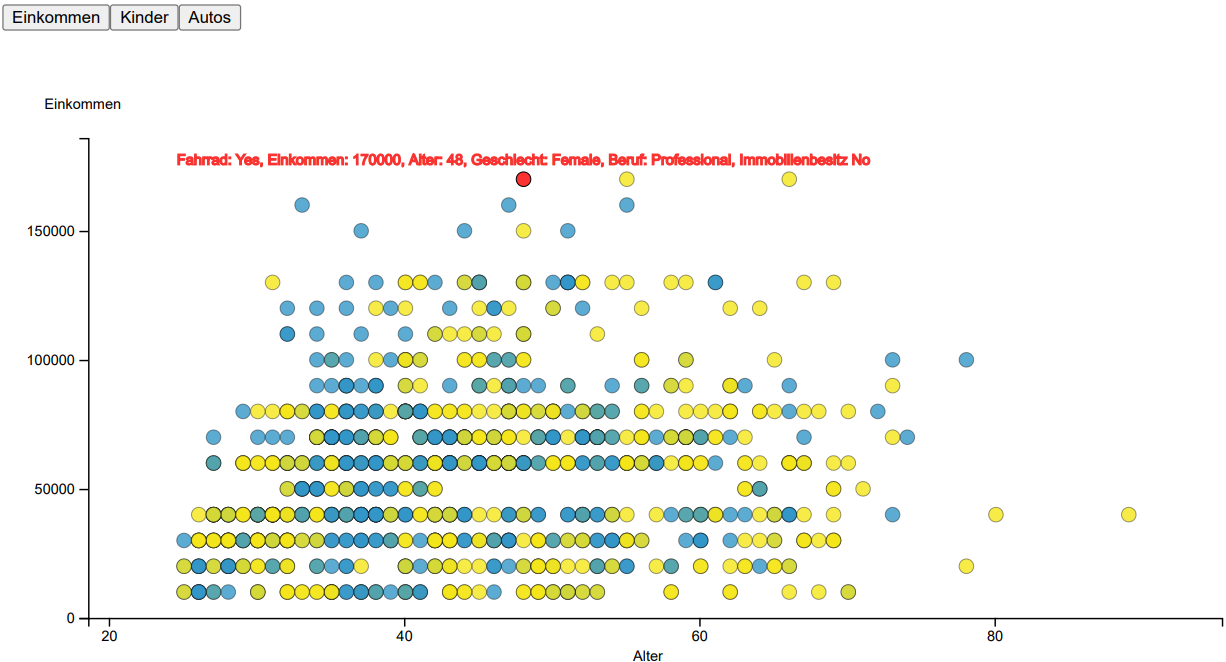
\includegraphics[width=16cm]{Bilder/V1Scatterplot.png}
\caption{Scatterplot für Fahrradkäufe, Quelle: Eigene Darstellung}
\end{center}
\end{figure}
\newline Die eingangs aufgestellten Scatterplot-Anforderungen konnten in der Abbildung 1 umgesetzt werden. Die beliebige Y-Achsenveränderung  erweitert die Anforderungen so, dass Anwendende den Darstellungsinhalt und Schwerpunkte selbst setzen können. Blaue Punkte symbolisieren, dass die befragte Person ein Fahrrad besitzt, während gelbe Punkte aussagen, dass die Person kein Fahrrad besitzt. Stärker sichtbare Punkte und jeweils kräftigere Blau- und Gelbtöne bedeuten, dass die Daten in diesen Punkten miteinander übereinstimmen. Punkte mit jeweils schwächeren Blau- und Gelbtönen zeigen in dieser Koordinatenumgebung weniger Übereinstimmung. Farbmischungen, wie die hellgrün eingefärbten Punkte, zeigen hingegen, dass hierbei sowohl Fahrradkäufe wie auch Nichtkäufe vorliegen. Der Punkt, über den gerade gehovert wird, ist für diese Aktion in der Farbe rot dargestellt. Die damit zusammenhängende rote Anzeige liefert die Zusatzinformationen zum Punkt.

Eine Alternative zur zweidimensionalen Darstellung stellen Zeitreihendiagramme dar, welche Zeitverläufe von Daten zeigen. Im Fahrradkaufdatensatz sind keine zeitlichen Ausprägungen vorhanden, weswegen der Scatterplot gewählt wurde.

\subsubsection{Visualisierung Zwei}
Mit den Parallelen Koordinaten können mehrdimensionale Zahlenwerte, gleichzeitig über vertikale Achsen, ohne X Achse mit Polygonlinien als Punktrepräsentation dargestellt werden.
Für die Fahrradkaufdaten besteht hier der Vorteil, gleichzeitig alle relevanten Zahlenwerte in einer Visualisierung darzustellen. Wie beim Scatterplot haben Anwendende die Möglichkeit die Darstellung über Buttons zu verändern. Diese können die Achsen beliebig miteinander vertauschen und neue Zusammenhänge, je nach Betrachtungsziel, hervorheben. 
\begin{figure}[h]
\begin{center}
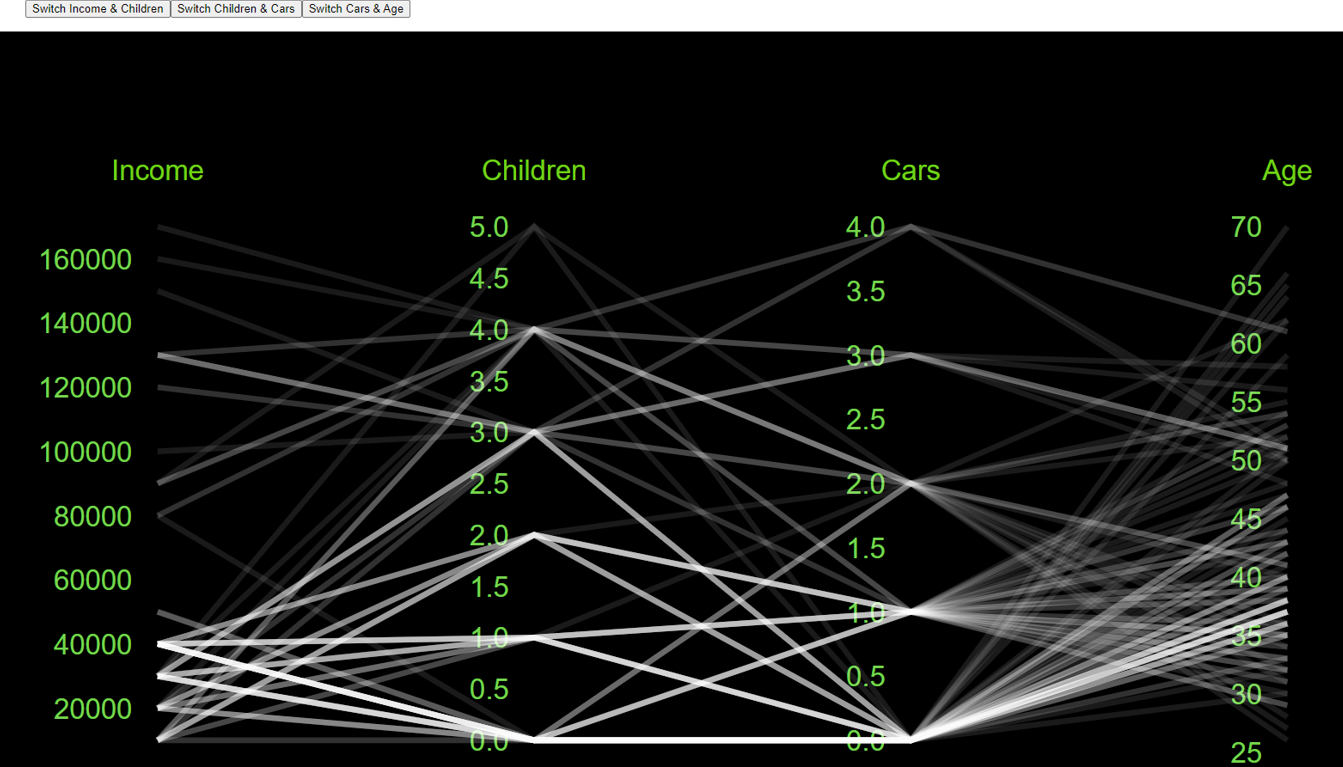
\includegraphics[width=16cm]{Bilder/V2ParalleleKoordinaten.png}
\caption{Parallele Koordinaten für die Fahrraddaten, Quelle: Eigene Darstellung}
\end{center}
\end{figure}
\newline Die Abbildung 2 zeigt von links nach rechts den Verlauf eines mehrdimensionalen Punktes beginnend mit dem Einkommen, der Kinder- und Autoanzahl und dem Alter der befragten Person. Der Vorteil im Vergleich zum Scatterplot ist, dass mehrere Zusammenhänge und Auffälligkeiten gleichzeitig erkennbar sind. Im Direktvergleich mit der Abbildung 1 gibt es keine Hoverfunktion, wodurch die Linien individuell nachverfolgbar wären, da diese den Fokus von der Musteridentifikation nehmen würde. Mit der Wahl des dunklen Hintergrunds und heller Linienfarbe ergibt sich eine Röntgendarstellung. Durch die Linienüberlappung werden Identifikationsmuster sichtbar, was sich durch die kräftigeren Weißtöne erkennen lässt. Darüber hinaus bieten die  Achsenbeschriftungen gute Anhaltspunkte für den Linienverlauf. Das Vorfiltern nach Region und Fahrradkauf im Elm-Programm verhindert eine Überdarstellung und Reizüberflutung für die Anwendenden. Somit wurden nicht nur alle Anforderungen aus der Einleitung abgeleitet, sondern auch die Gefahr der Übervisualisierung erkannt und verhindert.
Neben Parallelen Koordinaten gibt es weitere Visualisierungsmöglichkeiten mehrdimensionaler Daten. Da Scatterplots, am besten für zweidimensionale Daten geeignet, bereits verwendet wurden, stellen Projektion und Sektion, Sternkoordinaten, K-Means und Datentinte eine Alternative im Rahmen der Vorlesung zu Parallelen Koordinaten dar. Mit Projektionen und Sektionen soll der mehrdimensionale Raum abgebildet werden. Eine hierfür anfallende hohe Anzahl an benötigten Darstellungen kommt in Bezug auf die Übersichtlichkeit und Anwendungsfreundlichkeit für die Zielgruppen nicht in Frage. Mit Sternenkoordinaten können mehrdimensionale Daten in 2D oder in 3D abgebildet werden. Der Name ist charakteristisch für die Achsenanordnung. Auf Grund der ungewöhnlichen Erscheinung und der besseren intuitiven Nachvollziehbarkeit der Fahrradkaufdaten wurde auf die Parallelen Koordinaten zurückgegriffen. Die Visualisierungstechniken K-Means und Datentinte fokussieren die Visualisierung durch Vorabberechnungen auf wenige Kerngedanken und verhindern somit einen Überblick über eine breitere Sichtweise, welche für alle Zielgruppen anvisiert wurde, weshalb diese Alternative verworfen wurde.
\subsubsection{Visualisierung Drei}
Als dritte Visualiserungstechnik wurde die zu Beginn beschriebene Baumhierarchie ausgewählt, durch welche die Fahrradkäuferdaten geordnet werden. Die Knoten stellen hierbei Entscheidungsmöglichkeiten dar, welche durch die Linien miteinander verbunden werden. Die erste Unterscheidung besteht beim Fahrradkauf, wobei die Angaben in Ja oder Nein unterteilt werden. Anschließend erfolgt die Unterscheidung nach den Regionen der Personen. Die letzte Verzweigung stellt die Pendeldistanz vom Wohnort zur Arbeit dar. 
\begin{figure}[h]
\begin{center}
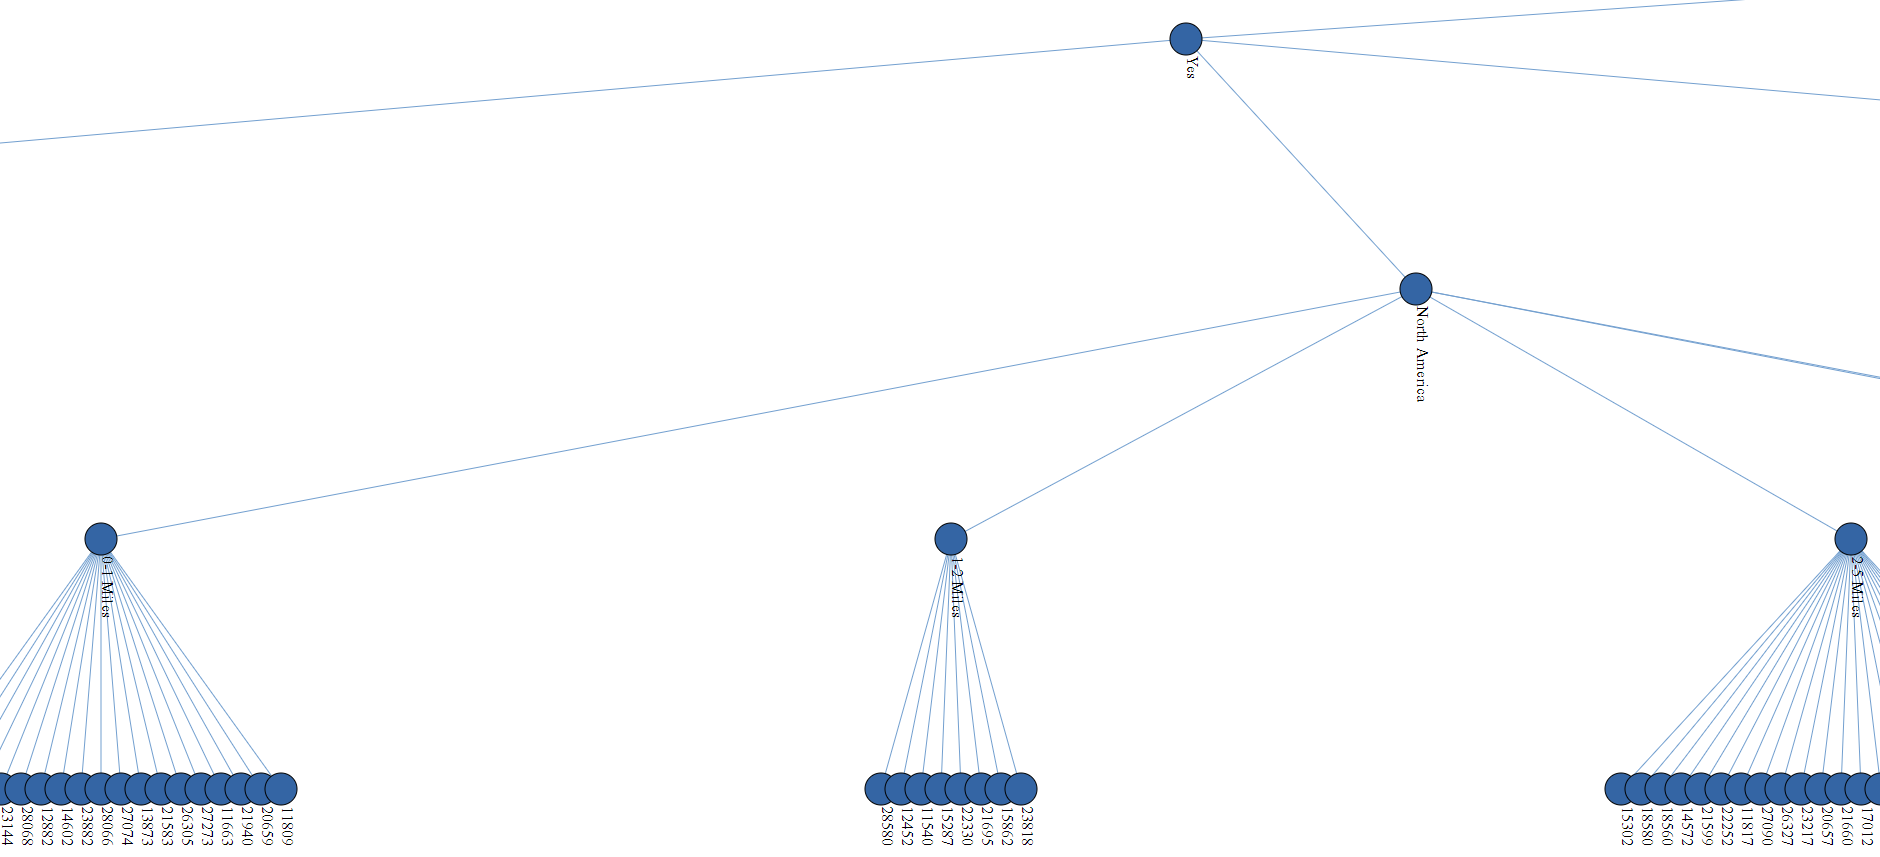
\includegraphics[width=16cm]{Bilder/V3Baumhierarchie.png}
\caption{Ausschnitt aus der Baumhierarchie für die Fahrraddaten, Quelle: Eigene Darstellung}
\end{center}
\end{figure}
\newline
Die Abbildung 3 zeigt einen Ausschnitt aus der umfangreichen Baumdarstellung. In der untersten Ebene sind die verschiedenen Pendeldistanzen aufgegliedert. Hierbei lassen sich die eingefärbten Knoten gut unterscheiden. Im Vergleich zu den beiden vorangegangenen Visualisierungen wurde auf eine Interaktionsmöglichkeit verzichtet. Die abgeleiteten Baumhierarchie-Bedingungen, also die übersichtliche Darstellung und Einteilung in Gruppen, konnten umgesetzt werden. Trotz Vorfilterung der Parameter, dass die Personen keine Autos besitzen, ist die Baumstruktur sehr umfangreich, weshalb auf weitere Unterteilungen, wie nach Familienstand, Beruf oder Bildungsstand verzichtet wurde. Diese werden teilweise durch die Hoverfunktion im Scatterplot ersichtlich. Neben der Möglichkeit die dritte Visualisierung als Baum darzustellen, gibt es in der Vorlesung weitere Kategorien, welche allerdings die Darstellung komplexer machen. Hierunter fallen verschiedene Graphenanwendungen, die Mehrfachzuweisungen auf Knoten ermöglichen. Auf Grund der Zielsetzung, die Infrastrukturplanung visuell intuitiv zu unterstützen und übersichtlich aufzuzeigen, welche Pendeldistanzen auftreten, wurde auf eine komplexere Darstellungsmethode verzichtet. 
\subsection{Interaktion}
Für die Visualisierungen Scatterplot und Parallele Koordinaten wurden zwei verschiedene Interaktionsmöglichkeiten in den jeweils zugrunde liegenden Code integriert. 

Bei der Visualisierung des Scatterplots haben Anwendende die Option, die Gegenüberstellung des Alters auf der X Achse mit einem beliebig verfügbaren Zahlenwert des Bike-Buyers-Datensatzes auf der Y-Achse  über das Klicken auf die verschiedenen Buttons anzeigen zu lassen. Dadurch kann der Fokus individuell auf bestimmte Sachverhalte gelegt werden, was insbesondere für Fahrradhersteller und Fahrradhändler interessant ist. Um die eingeschränkte Funktionalität der zweidimensionalen Zahlengegenüberstellung zu erweitern, wurde die Hover-Funktion integriert. Durch das Hovern über den Punkten des aufgespannten Koordinatensystems werden auch Textdaten als Informationen, wie der Beruf oder Immobilienbesitz ausgegeben. Daneben lassen sich die exakten Datenwerte beim Einkommen anzeigen, welche lediglich als Achseneinteilung zu ungenau wären. 

Die zweite Visualisierung, Parallele Koordinaten, bietet Interessenten die Möglichkeit über Buttons die Achsen nach belieben zu verschieben. Je nach Einstellung lassen sich Zusammenhänge der Polygonlinie hervorheben, was durch eine eindeutigere Überlappung der hellen Linien sichtbar wird. Anwendende werden dadurch ermutigt, selbst die Daten in eine für sie interessante Sichtweise zu verschieben, was beispielsweise bei Verkaufstrainings für den Fahrradhandel, aber auch für zielgerichtete Kundenwerbung hilfreich ist. 

Für das Baumdiagramm wurde auf eine Interaktionsmöglichkeit verzichtet, da das Visualisierungsziel über die Ebenendarstellung erfüllt ist. 

Über die Startseite "`index.html"' kann aus dem eigenen, öffentlichen Github Repository eine \href{https://floeagle.github.io/Bike-Buyers-1000/index.html}{\textbf{Website}} dargestellt werden. Dabei wurden die drei Visualisierungen als HTML-Seite, hervorgerufen durch den Terminalbefehl in VSC "`elm make"', jeweils verlinkt. Untereinander sind die HTML-Seiten miteinander vernetzt, sodass eine Interaktion möglich ist. Dabei können Anwendende, je nach Anwendungsziel, beispielsweise einen Zusammenhang im Scatterplot auf mehrdimensionaler Ebene mit Hilfe der Parallelen Koordinaten oder andersrum untersuchen, indem sie auf dafür konfigurierte Buttons zwischen den drei Visualisierungen und der Startseite wechseln können.
\section{Implementierung}
Die Ausgangsbasis für die Funktionsweise der Visualisierungen auf Codeebene  stellen die Programmcodes mit ihren Funktionen aus der Übung dar. Für die Scatterplot-Visualisierung wurden die im Rahmen der Übungen eins bis drei entwickelten Codegerüste als Grundlage verwendet. Für die Parallelen Koordinaten ist die Übung sieben der Ausgangspunkt. Bei der Baumhierarchie galt die Übung zehn als Orientierung. 
%Beschreibung der einzelnen Programme
%Scatterplot
Alle drei Visualisierungsprogramme beginnen mit dem Importieren der für die jeweiligen Elm-Programme notwendigen Pakete. Es wurden keine eigenen Module eingesetzt. Ein Überblick über alle verwendeten Pakete ist in der Readme.md im Github-Repository einsehbar. 

Im Scatterplot-Code folgen als nächstes Funktionen, welche die Darstellung für die spätere Scatterplot-Funktion, wie die Achsen oder die Größe, konfigurieren. Direkt im Anschluss folgen type-Festlegungen zur Weiterverwendung in Funktionen der Elm-Datenstruktur, welche die Y-Achsenwerte definieren. Die main-Funktion zeigt die Codegliederung der Elm-Datenstruktur auf.
Die init-Funktion legt die erste dynamische Scatterplot-Variante aus "`Alter"' und "`Einkommen"' fest. Die update-Funktion bestimmt den Darstellungswechsel über die Y-Achse. Als Teil der Elm-Struktur werden subscriptions für die main-Funktion gebraucht. Mit view wird die HTML-Seite, inklusive Start- und Buttoninteraktion, angezeigt. Die nächsten drei Funktionen dienen der Visualisierungsspezifikation der Scatterplot-Punkte und der Scatterplot-Funktion.
Anschließend kommen Funktionen, welche die Möglichkeit zulassen sollen, den Datensatz beliebig zu skalieren und auch leere Werte im Programm zu filtern. Als letztes finden sich Funktionen für das Decoden des großen CSV-Strings, welcher sich am Ende der Datei befindet. Diese letzten beiden Gliederungsfunktionen sind identisch mit dem Programm für die Parallelen Koordinaten. 
%Parallele Koordinaten
\newline Im Programm für die Parallelen Koordinaten findet sich der gleiche Aufbau wieder. Nach den Paketimporten, der Darstellungskonfiguration der Parallelen Koordinaten und den type-Funktionen zur Verwendung in der Elm-Datenstruktur wird im init die Startvisualisierung mit der Achsenreihenfolge festgelegt. Die beiden Funktionen indexSwap und update sind für den Achsenwechsel und die dafür notwendige Festlegung der Reihenfolge verantwortlich. 
Im let-Block der view-Funktion werden zwei Parameter der Fahrraddaten vorgefiltert, um die Polygonlinien sichtbar darzustellen. Die view Funktion verwaltet die auf der HTML Seite dargestellten Inhalte. Über die parallelCoordinatesPlot-Funktion wird die Abbildung der vertikalen Achsen organisiert und über die Funktion colordescr die Achsenfarbe und Darstellung angepasst. Die letzten Funktionen dienen dem Herausfiltern potenziell zukünftig fehlender Werte und der Csv-String-Decodierung. 
%Baumhierarchie
\newline Bei der Baumhierarchie wird im init, nach dem Paketimport, der type-Festlegung und dem Konfigurieren der Elm-Datenstruktur über main, der vorbereitete Link zur JSON-Datei in das Programm geladen. Das Update dient zur Baumdarstellung würde im Fehlerfall eine Benachrichtigung anzeigen. Danach folgen Funktionen zur Knotenfestlegung und Kantendarstellung, sowie Layout-Konfigurationen. Nach der view-Funktion für die HTML-Anzeige unter Berücksichtigung der Konfigurationsfunktionen befindet sich der JSON-Tree-Decoder, welcher die als "`id"' gespeicherten Fahrraddatenwerte aus der verlinkten JSON-Datei als Textwert entpackt. 



%Decoder
Für die ersten beiden Visualisierungen wird ein CSV-Decoder benötigt. Während der Projekt-Konzeptionsphase wurde versucht, mit Hilfe des CSV-Decoders nach dem Vorbild aus Übung acht die Daten in das Elm-Programm zu laden. Allerdings ist der unübersichtliche Aufbau des Decoders nicht für die Projektarbeit mit den Fahrraddaten geeignet. Hierzu sind weitere Decoder-Funktionen notwendig, die zur Komplexität und Unübersichtlichkeit der Elm-Codes beitragen.
Da in der Entwicklungsphase des Projektes viele Codeanpassungen erfolgen, ist die Linkaktualisierung im Vergleich zu den im Kapitel 2.1 beschriebenen Vorteilen durch einen CSV-String nicht gewünscht. Deshalb wurde ein geeignetes Decoder-Paket für Elm in der offiziellen Dokumentation gesucht.
Ein Vorbild stellten hierzu die IRV-Car-Übungen mit den darin gespeicherten Daten dar. Der Unterschied ist, dass diese Car-Daten "`elmgerecht"' aufbereitet wurden, wodurch eigene Datentypen über type problemlos zum Filtern festlegbar sind. Zusätzlich sind die CSV-Daten in Elm nicht ohne Decoder-Funktionen einlesbar. Der Entwickler Brian Hicks bietet einen für die Anforderungen an die Fahrraddaten passenden Decoder. Dessen Paket für Elm wurde in die beiden Elm-Programme Scatterplot und Parallele Koordinaten importiert und die Decoder-Funktion aufgebaut. 
Die Herausforderung in dieser Phase war die Decoder-Implementierung, sodass das Elm-Programm die Fahrraddaten richtig laden und darstellen kann. Nach erfolgreichen Tests dieser Anforderung wurde mit der zweiten Phase begonnen.

Diese Phase umfasst die Verbindung der decodierten Fahrraddaten mit den Codegerüsten aus der Übung zum Scatterplot und zu den Parallelen Koordinaten. Die nötige Konfiguration von Datentypen, das Einbinden des Decoders in die main-Funktion, sowie die Anpassung des Scatterplots und der Punkte (richtige Farbe, Anzeige, Hover-Interaktion mit den Punkten) stellten eine Herausforderung dar, die durch "`Try and Error"' bewältigt werden konnte. Die gemachten Erfahrungen mit der Verknüpfung zwischen Decoder und Codegrundgerüst konnten gut auf die Programmierung der Parallelen Koordinaten übertragen werden, sodass die Grundfunktionsweise (keine Interaktionsmöglichkeit mit der Anwendung) erfolgreich angewendet werden konnte. Nach Tests zu der Röntgendarstellung der Linien im Vergleich zu "`normaler"' Darstellung wurde die Röntgendarstellung für die zweite Visualisierung gewählt.
Für die Baumhierarchie stellte die erste Phase die Datenvorverarbeitungsschritte für die JSON-Datei dar. In der Übung 10 wurde ebenfalls ein JSON-Decoder verwendet, sodass keine nennenswerten Komplikationen mit dem Lesen der JSON-Datei auftraten. In der zweiten Phase wurde das default-Layout durch eine eigene Layout-Funktion ersetzt, wozu zunächst der Elm-Paketimport erweitert wurde.
%DRITTE pHASE
Die dritte Phase umfasste das Programmieren von Interaktionsmöglichkeiten mit der Anwendung, wie die Buttons zum Wechseln der Y-Achsen beim Scatterplot und den Achsentausch der Parallelen Koordinaten. Eine Herausforderung stellte die dafür notwendige Anpassung der Programmgliederung dar, was nicht nur durch die oben genannten Übungen als Anhaltspunkt, sondern ebenfalls durch Ausprobieren und Recherche in den Elm-Dokumentationen funktionierte. 
Um die drei Visualisierungsdateien miteinander zu verbinden, wurde der "`elm-make"'-Befehl verwendet und die Dateien untereinander und mit einer "`index.html"' Seite verknüpft, die als Startseite der Anwendung dient. Hierbei war eine regelmäßige Iteration notwendig, um in den jeweiligen Programmen vorgenommene Änderungen zu aktualisieren. 
 
\section{Anwendungsfälle}
Im folgenden werden für die drei Darstellungen in Hinblick auf die Zielgruppe praktische Anwendungsfälle aufgezeigt. 
\subsection{Anwendung Visualisierung Eins}
In der Abbildung 4 ist ein Scatterplot mit der Achsenauswahl "`Alter"' zu "`Autos"' abgebildet, welcher sich besonders an die Zielgruppe des Fahrradhandels richtet.
\begin{figure}[h]
\begin{center}
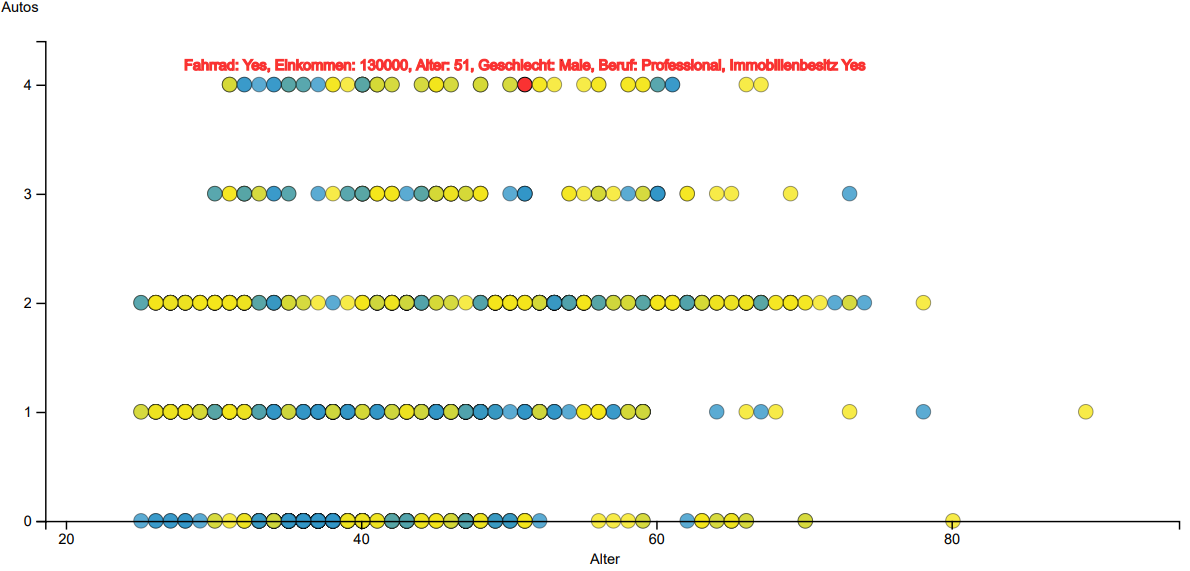
\includegraphics[width=16cm]{Bilder/ScatterplotA1.png}
\caption{Anwendung Scatterplot, Quelle: Eigene Darstellung}
\end{center}
\end{figure}
\newline Aus dieser Konfiguration lassen sich einige Informationen entnehmen, welche dabei helfen können, die Kundenzielgruppe besser einzuordnen. Aus diesen Informationen können beispielsweise im Rahmen von Schulungen Kundenfragen abgeleitet werden, deren Antworten dabei helfen können, Kaufinteressierte besser einzuordnen. 
So lässt sich erkennen, dass hauptsächlich Personen zwischen Ende 20 und Mitte 50 kein Auto und mehrheitlich ein Fahrrad besitzen. Diese Altersgruppe entspricht demographisch auch stark der berufstätigen Bevölkerung. Des weiteren haben Personen mit vier Autos tendenziell weniger Fahrräder. Auffällig wenige befragte Personen mit zwei Autos haben kein Fahrrad. Zusammenfassend lässt sich interpretieren, dass der Besitz mindestens eines Autos einen negativen Einfluss auf den Fahrradbesitz hat. 
Personen mit vielen Autos werden voraussichtlich entsprechende Stellplätze zur Verfügung haben, wo sie platzsparender für verschiedene Einsatzbereiche (wie Baustelle im Stadtverkehr oder Autoreparatur) ein Fahrrad als Alternative zum Auto abstellen könnten. 
Die Personengruppe mit vier Autos hat bis auf eine Ausnahme Berufe im Management und in spezialisierten Fachbereichen. Bei den Personen ohne Auto sind die Berufsgruppen gemischt, wobei viele Büroangestellte oder tätig im Handwerk sind.
Durch die Zusatzinformation zum Eigenheimbesitz können ebenfalls Rückschlüsse auf Einkommen, verfügbaren Platz und die Bereitschaft mehr für ein Fahrrad auszugeben, gezogen werden. Hier besteht für den Fahrradhandel die Möglichkeit Rabatte auf den Kauf weiterer Fahrräder für verschiedene Verwendungsbereiche anzubieten.

Um diese Zusammenhänge aufzuzeigen kommt als Alternative nur bedingt die Darstellung über Parallele Koordinaten in Frage. Über die stärker hervortretenden Polygonlinien der Röntgendarstellung ist erkennbar, dass jüngere Leute überwiegend kein Auto haben. In dieser Visualisierung können allerdings keine Werte eindeutig voneinander getrennt betrachtet werden. Darüber hinaus sind über die verschiedenen Farbakzente der Punkte und Zusatzinformationen beim Hovern Funktionsweisen mit dem Scatterplot verbunden, die über keine Darstellungsalternative zu ähnlich qualitativen Ergebnissen kommen würden.  

\subsection{Anwendung Visualisierung Zwei}
Die zweite Anwendung stellt die in Abbildung 5 gezeigte Achsenumstellung dar. Diese ist besonders für Fahrradhersteller geeignet, weist aber auch Eigenschaften auf, die für den Fahrradhandel interessant sind. Im dazugehörigen Elm-Programmcode wurden Daten gefiltert, die "`Yes"' zum Fahrradkauf und als Region "`Europe"' angeben haben. Durch die erste Filterung lässt sich für die Fahrradhersteller besser erkennen, was nachgefragt wird. Die zweite Vorfilterung wurde vorgenommen, damit der Datensatz auf Grund zu vieler Daten nicht unübersichtlich wird. Die meisten Datenwerte sind für die Region Nordamerika verfügbar. Danach folgen in Abstufender Reihenfolge Europa und Pazifik. Europa wurde auf Grund des Regionalbezugs und der damit einhergehenden Assoziation für regionale Unternehmen gewählt.
\begin{figure}[h]
\begin{center}
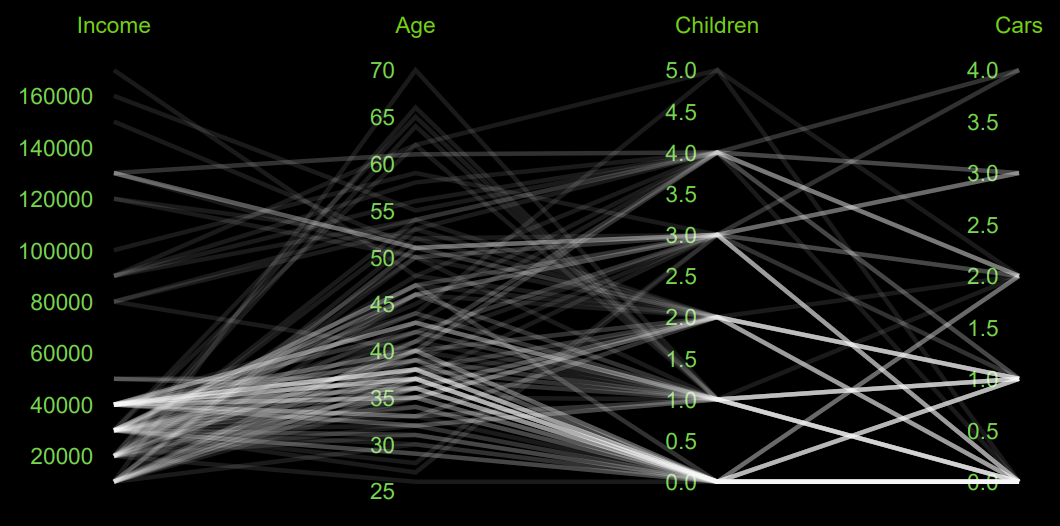
\includegraphics[width=16cm]{Bilder/ParallelCoordsA2.png}
\caption{Anwendung Parallele Koordinaten, Quelle: Eigene Darstellung}
\end{center}
\end{figure}
\newline In der Abbildung zeigt sich, dass die Mehrheit, der vorgefilterten Fahrraddaten ein im Vergleich zu den Einkommensachsenwerten geringes Einkommen aufweisen und dass dieses mit zunehmendem Alter steigt. Überwiegend jüngere Personen zwischen 30 und 40 haben keine Kinder. Ältere Personen haben tendenziell mehr als ein Kind und dementsprechend bereits viele Kinderfahrräder gekauft. Im Umkehrschluss könnten Fahrradhändler jüngeren Personen mit wenigeren Kindern auch mehr zusätzliche Kinderfahrräder verkaufen, da diese noch nicht an jüngere Geschwister übergebbar sind.
 Im Hinblick auf die in 1.1 geschilderten Zusammenhänge können Fahrradhersteller  für ältere Personen höherpreisige Fahrräder herstellen, welche die angesprochenen Eigenschaften, wie bessere Abstiegsmöglichkeiten durch niedrigere Gabel oder schmalere Griffe besitzen und neue Technologien verwenden. Gleichzeitig bedeutet es, dass Hersteller für eine jüngere Zielgruppe preiswertere Fahrräder herstellen sollten, da diese, wie in Abbildung 5 ersichtlich mehr Fahrräder kaufen als ältere.  

Durch die Parallelen Koordinaten können übersichtlich Trends und Verallgemeinerungen abgeleitet werden, ohne vorher einen Bereich hervorzuheben.  
Diese intuitive Beobachtung ist am ausdrucksstärksten in Kombination mit dem Scatterplot. Durch den Direktvergleich der beiden Visualisierungen fusionieren die Stärken beider Anwendungen. Beispielsweise lassen sich Muster erkennen, wie dass Personen mit vier bis fünf Kindern ein höheres Einkommen haben. Für Fahrradhersteller ist außerdem die genaue Hoveranzeige in Verbindung mit dem Scatterplot interessant, da hier zusätzlich Informationen zum Geschlecht eingeholt werden können. Die aus der Projektanforderung und der Vorlesung abgeleiteten Visualisierungsalternativen wie Projektion und Selektion, K-Means oder Datentinte kamen auf Grund der zu starken Fokussierung auf individuelle Zusammenhänge in zahlreichen Zusatzdarstellungen nicht in Frage. Dafür wären Zusammenhänge, wie zwischen Einkommen und dem Preis des gekauften Fahrrads geeignet, die im Datensatz nicht vorliegen. Die Sternenkoordinaten würden zu viel Zeit zum Nachvollziehen der ungewöhnlichen Struktur benötigen und würden die Zusammenhänge zu grob darstellen. Aus diesen Gründen wurden die Parallelen Koordinaten gewählt. 

\subsection{Anwendung Visualisierung Drei}
\begin{figure}[h]
\begin{center}
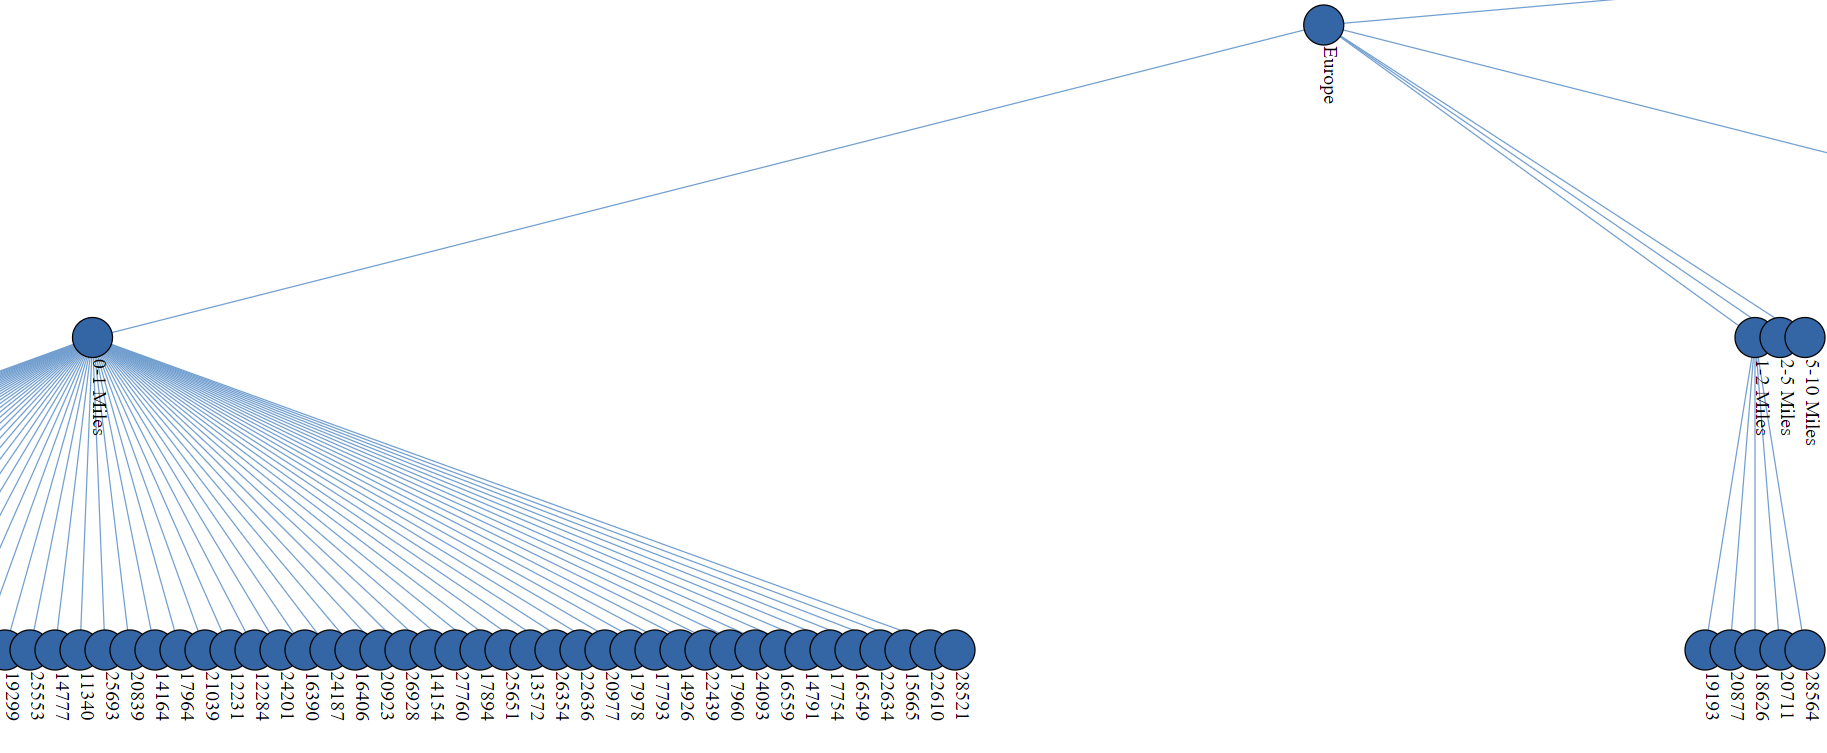
\includegraphics[width=16cm]{Bilder/BaumhierarchieA3.png}
\caption{Anwendung Baumhierarchie, Quelle: Eigene Darstellung}
\end{center}
\end{figure}
Aus der Abbildung 6 geht hervor, dass in Europa von den Fahrradkaufenden ohne Auto die überwiegende Mehrheit eine geringe Distanz von Zuhause zur Arbeit aufweist. Da diese Distanz für den öffentlichen Nahverkehr zu gering wäre, gleichzeitig aber Distanzen von 1.6 Kilometer (eine Meile) nicht mehr zeitsparend und ohne Anstrengung zu Fuß zu bewältigen sind, kann davon ausgegangen werden, dass viele dieser Fahrradkaufenden das Fahrrad für den Arbeitsweg verwenden. Auf Grund der kurzen Entfernung ist anzunehmen, dass die Daten in Großstädten gesammelt wurden. Die Infrastruktur ist in diesen häufig von mehrspurigen Straßen mit vielen unübersichtlichen Kreuzungen und Abbiegungen gekennzeichnet. Infrastrukturprogramme, wie in der Einleitung beschrieben, sehen hierzu vor, dass besonders Fahrradwege besser ausgebaut werden sollen, damit weniger Verkehrsunfälle mit Fahrrädern passieren. Gerade deshalb ist dieser Ausschnitt aus der Baumhierarchie für in Frage kommende Bauunternehmen spannend. Daran lässt sich erkennen, dass vermeintlich kurze Distanzen für Fahrradwege zwischen bereits vorhandener Infrastruktur gebaut werden müssen, um zu einer klimaneutralen, sicheren und verkehrsberuhigten Innenstadt beizutragen. 
Andere Darstellungsmethoden, die im Anforderungs- und Vorlesungsrahmen für eine vergleichbare Darstellung in Frage kämen, wie die Graphendarstellung, würden zur Unübersichtlichkeit der Verzweigungen auf Grund der großen Datenmenge beitragen. Deshalb ist die Baumhierarchiestruktur für diesen Sachverhalt, nämlich das Aufzeigen der verschiedenen Pendeldistanzen, optimal gewählt. 
\newpage
\section{Verwandte Arbeiten}
Zum Themenbereich Fahrrad und damit verbundenen Entwicklungen wird eine Auswahl an Publikationen vorgestellt, welche vergleichbare Visualiserungstechniken zu diesem Forschungsbericht verwendet haben. 

Eine Forschungsarbeit zum Thema Nutzungsverhalten von E-Bikes greift unter anderem auf Scatterplots zurück, um Zusammenhänge zwischen mit E-Bikes zurückgelegten Kilometern und gutem Wetter aufzuzeigen \cite{Rios.06212016}. Ein weiteres Projekt zur Untersuchung des Fahrradverleihs im südkoreanischen Seoul zeigt unter Einsatz der Scatterplot-Technik, dass ein Zusammenhang zwischen hohen Temperaturen und erhöhter Anzahl an vermieteten Fahrrädern besteht und dass bei hohen Windgeschwindigkeiten weniger Fahrräder ausgeliehen werden \cite{Kashyap.2021}. Gemeinsamkeiten zu diesen beiden Arbeiten liegen in der Verwendung der gleichen Visualisierungstechnik und dem Aufzeigen von damit verbundenen Interpretationen. Anders als bei den verwandten Arbeiten wird in diesem Bericht auch die Interaktion mit der Visualisierung ermöglicht. 

Des weiteren existiert eine Arbeit zur Informationsvisualisierung, die sich auf die Visualisierung von Gemeinsamkeiten und Unterschieden zwischen Fahrradverleih und Taxiservice konzentriert. Hierbei wird eine Anwendung bereitgestellt, mit der interagiert werden kann. Über Buttons kann die Ansicht zwischen einem Hierarchieüberblick, Liniengraphen zu Zeitverläufen und zwei Stadtkarten-Heatmaps für Serviceregionen gewechselt werden. Für den Hierarchieüberblick wurde anstelle eines Baumdiagramms ein Sunburst-Diagramm verwendet, da hierbei ein sehr großer Datensatz mit wenig Platz abgebildet werden kann. Neben den erwähnten Buttons ist die Interaktion mit der Vergleichsanwendung tiefgreifender. So haben Anwendende die Möglichkeit, in der Hierarchie zu filtern, Muster direkt auszuwählen, und die Daten über eine Navigationszeile in eine beliebige Reihenfolge zu bringen. Darüber hinaus können erkannte Muster erstellt, benannt und andere Muster gelöscht werden. Über Mausinteraktionen kann aus der Anwendung heraus- und hineingezoomt werden. Ähnlich wie die Hoverfunktion bei den Scatterplots dieser Arbeit kann beim Hovern über die Sunburst Hierarchie der Sektor hervorgehoben werden. Diese Forschungsarbeit weist detailliertere Interaktionsmöglichkeiten als dieser Bericht zu den Fahrradkaufdaten auf. Ein Ziel dieser verwandten Arbeit von Dai et al. \cite{Dai.2020}, nämlich die Stadtplanung zu verbessern, überschneidet sich mit dem Visualisierungsziel des Baumdiagramms dieser Arbeit, die Planung der Fahrradweginfrastruktur von involvierten Bauunternehmen zu unterstützen. 

Eine weitere Studie zu öffentlichen Fahrradverleih-Systemen, mit Interaktionsmöglichkeiten, verwendet verschiedene Weiterentwicklungsmöglichkeiten der  Parallelen Koordinaten. In der Standardvariante werden ebenfalls Attribute gegenübergestellt. In der beschriebenen Arbeit werden allerdings fünf Achsen verwendet. Mit deren Anwendung können Nutzer eigenständig Daten filtern und durch Hovern über die Linien, welche die Parallelen Koordinaten verbinden, werden die jeweiligen Linien hervorgehoben. Des weiteren sind einige Linien in Farbe hervorgehoben, was auf weitere Muster hindeutet. Grundsätzlich gemeinsam mit diesem Ansatz ist, dass die Daten gefiltert werden. Der Unterschied in dieser Arbeit ist, dass die Daten im Elm-Code vorgefiltert wurden und nicht durch Visualisierunsanwendende. Zusätzlich kann in der verwandten Arbeit über das Hovern die jeweilige Linie hervorgehoben werden, was in dieser Forschungsarbeit nicht implementiert wurde. Somit stellen die Unterschiede die Achsenanzahl, die farbigen Linien im Vergleich zum Kontrast der Röntgendarstellung, die Filteranwendung durch Nutzende und das Hovern dar \cite{Shi.2018}.  
\section{Zusammenfassung und Ausblick}

Dieses Projekt konnte die Datenaufbereitung zu einem sehr aktuellen Thema visuell umsetzen. Die Aktualität wird durch die vermehrte Ausstellung von Fahrrädern auf der zeitgleich zur Projektabgabe stattfindenden IAA Mobility in München deutlich \cite{.08.09.2021}.

Durch den Scatterplot konnten Zusammenhänge aufgezeigt werden, welche insbesondere für die Zielgruppe des Fahrradhandels interessant sind. Trotz der Limitation, dass lediglich zwei Daten über die X und Y Achse gegenübergestellt werden, ermöglicht die Hover-Interaktion genügendFreiraum für die Anwendenden, eigene Muster zu erkennen und für engere Kundenbindungen im Fahrradverkauf zu übertragen. 
Des Weiteren können Fahrradhersteller mit der Visualisierungstechnik der Parallelen Koordinaten interagieren, sowie Informationen und Muster (z.B. Einkommen, Alter) erkennen, welche bei der Fahrradproduktion unterstützen können.

Die dritte Visualisierung ermöglicht es einen komplexen Sachverhalt übersichtlich und ohne notwendige Vorkenntnisse aufzuzeigen, der intuitiv verständlich ist. Über die Baumhierarchie wird die Relevanz für kurze Fahrradwege sichtbar.
Besonders in Großstädten ist diese Thematik brisant, da hier im Verkehr häufig Fahrradunfälle passieren \cite{Reek.17.03.2021,Nogly.2014,tagesschau.20.08.2021}. Deshalb eignet sich diese Visualisierung für Bauunternehmen im Bereich der Fahrradwege-Infrastruktur und alle an der Planung und dem Bau beteiligten Gruppen.

Somit löst dieses Projekt die Herausforderung den Anforderungen mehrerer Zielgruppen gleichzeitig gerecht zu werden.   
Im Bezug auf Interaktionen stellen folgende Inhalte eine Weiterentwicklung dar. Die Hauptwebsite index.html könnte noch ansprechender visualisiert werden, wie beispielsweise durch ein Austauschforum für Anwendende. Einen weiteren Punkt stellen die Interaktionsmöglichkeiten für Anwendende dar, welche so erweitert werden könnten, dass Nutzende selbst die Möglichkeit haben die Daten nach Region, bestimmten Werten oder Wertschwellen, sowie individuellen Parametern über Buttons zu filtern. Dies würde die Zielgruppe nochmals erweitern, sodass nicht nur europäische sondern auch amerikanische oder pazifische Branchenunternehmen angesprochen werden. Die Interaktion im Bereich der Parallelen Koordinaten könnte ebenfalls Hoverfunktionen beinhalten, wozu die parallelCoordinatesPlot-Funktion im in-Bereich angepasst werden müsste. Im Rahmen dieses Projekts wurde auf diese Anpassung verzichtet, da Zusatzinformationen über das Hovern im Scatterplot verfügbar sind und den Fokus zu sehr auf das Hovern lenken.

Aus Visualisierungssicht könnten mehr Visualisierungstechniken, wie die Sternenkoordinaten oder bei der Erhebung zeitlich abhängiger Fahrraddaten (gefahrene Kilometer pro Woche, etc.) Zeitdiagramme, verwendet werden, welche als zusätzliche Interaktionsmöglichkeit verknüpft sein sollten. Auch eine Option zum Ein- und Ausschalten der Röntgenansicht könnte für die Parallelen Koordinaten sinnvoll sein. 

Auf Datenebene könnten Erhebungen zur Häufigkeit des Fahrradfahrens, verwendetem Equipment wie Helme oder zusätzliche Beleuchtung, Verkehrssicherheit und Fahrstil interessant sein, um zusätzliche Gadgets zu verkaufen oder auch die Zielgruppe der Versicherungsbrache anzusprechen. Diese Daten könnten durch Umfragen erhoben und die Visualisierungen im Rahmen zukünftiger Forschungsprojekte erweitert werden.  

Zusammenfassend bereitet diese Forschungsarbeit zur Visualisierung von Fahrradkäufen im B2C-Segment für die Anbieterseite über die verschiedenen Darstellungstechniken Zusammenhänge, wie Einkommen, Alter und die Autoanzahl, die zum Fahrradkauf führen, auf. Diese sind für die beiden Zielgruppen Fahrradhersteller und Fahrradhandel mit dem aufgeführten Mehrwert verbunden. Wie durch die Baumdarstellung ersichtlich, stehen mit dem Fahrradboom besonders Kurzstrecken im Fokus, welche im Zusammenhang mit Infrastrukturprogrammen ausgebaut werden sollten. 
Mit der verfügbaren Zeit für die Projektarbeit, der zur Verfügung stehenden Ressourcen und Knowhow konnten für die Zielgruppen detaillierte Informationen und Zusammenhänge visualisiert werden. 
\newpage
\section*{Anhang: Git-Historie}
Das mit dem Bericht verbundene \href{https://github.com/floeagle/Bike-Buyers-1000}{\textbf{Github-Repository}} des Autors liefert detaillierte Einblicke in die Projektentwicklung. 
\begin{verbatim}


* 2b6e0c5 (HEAD -> main, origin/main, origin/HEAD) (Update d.dat, 2021-09-07)
*   5ad824b (Merge branch 'main' of https://github.com/floeagle/Bike-Buyers-1000 into main, 2021-09-07)
|\
| * 1f42099 (Delete Alte HTML Versionen directory, 2021-09-07)
* | 4689e49 (Anpassung gitignore, 2021-09-07)
|/
* 61359dc (Create .gitignore, 2021-09-07)
* 4d6e252 (Überarbeitung Kapitel 5, 2021-09-07)
* 2f164d0 (Verbesserung Kapitel 5 Anwendungen, 2021-09-07)
* af496a2 (Verbesserung Kapitel 4, 2021-09-07)
* b48d30a (Verbesserung Gliederung Parallele Koordinaten, 2021-09-07)
* 1f53f73 (Verbesserung Kapitel 3.4, 2021-09-06)
* 5aa43a5 (Verbesserung Kapitel 3.3.3, 2021-09-06)
* c8ae15f (Verbesserung Visualisierungskapitel der Parallen Koordinaten, 2021-09-06)
* 87d5a54 (Umgliederung ELM Codes, 2021-09-06)
* 1c545f4 (Verbesserung Kapitel 3.3.1, 2021-09-06)
* ad1b137 (Korrektur Zitierstil, 2021-09-06)
* 074f255 (Verbesserung Kapitel 2.2, 2021-09-05)
* 80fb135 (Überarbeitung Kapitel 2.1, 2021-09-05)
* c0ab931 (Verbesserung Satzbau Einleitung, 2021-09-05)
* 065eaff (Verbesserung Einleitung, 2021-09-05)
* 74bb576 (Überarbeitung Kapitel 1/2, 2021-09-05)
* 7b2fe28 (Update d.dat, 2021-09-05)
* 224a70d (Anpassung HTML Seite, 2021-09-05)
* 04c8453 (Anpassungen Baumhierarchie, 2021-09-05)
* 9afe259 (Verbesserung Baumdarstellung, 2021-09-05)
* d41f131 (Anpassung Text, 2021-09-04)
* 8bafa23 (Verbesserung Visualisierungen, 2021-09-04)
* b74498a (Überprüfung Parallele Koordinaten Daten, 2021-09-04)
* c5c9725 (Update d.dat, 2021-09-04)
* bf1c2ce (Fehlerbehebung Verlinkung und Dateienbezeichnung, 2021-09-04)
* eb239d4 (Fehlerbehebung, 2021-09-04)
* a831405 (Hoveranpassung Parallele Koordinaten, 2021-09-04)
* bd8cc04 (Ordneraktualisierung, 2021-09-04)
* e10b3cc (Aktualisierung HTML Links, 2021-09-04)
* 556dff6 (Experimentieren mit Farben, 2021-09-04)
* d69d965 (Ordner Neustrukturierung, 2021-09-04)
* 4d1c83f (Link Aktualisierung, 2021-09-04)
* 84ba535 (Anpassung Links, 2021-09-04)
* 93ab761 (Umbenennung Link, 2021-09-04)
* 5e706dc (Konfiguration HTML Seite, 2021-09-04)
* 33df469 (Anpassung Beschriftung filterMissingValues, 2021-09-04)
* 126fa10 (Korrektur ic Funktion zu farbe2Buyers, 2021-09-04)
* 0ff4e5c (Anpassung Code Scatterplot, 2021-09-04)
* 35d61f8 (Angleichung Code Scatterplot / Parallele Koordinaten, 2021-09-04)
* ea8c984 (Überarbeitung Code für Scatterplot, 2021-09-04)
* 93a8c9c (Überarbeitung Kapitel 2, 2021-09-04)
* 938ddfc (Verbesserung Überblick Einleitung, 2021-09-04)
* 7b79fbd (Überarbeitung Kapitel Zielgruppe, 2021-09-04)
* 0474a3f (Überarbeitung Anwendungshintergrund, 2021-09-04)
* bd6ec9e (Verbesserungen Einleitung und Kapitel Zielgruppe, 2021-09-03)
* 4066ee3 (Verbesserung Kapitel 1.2 Anwendungshintergrund, 2021-09-03)
* 4512e34 (Verbesserung Einleitung, 2021-09-03)
* d596f18 (Überarbeitung Einleitung, 2021-09-02)
* 3c55230 (Überarbeitung Einleitung, 2021-09-02)
* 75c785f (Fehlerbehebung, 2021-09-01)
* 185eb9f (Ausgestaltung der Readme, 2021-09-01)
* 4fdbd60 (Ergänzung benötigter ELM-Packages, 2021-09-01)
* c6aa58f (Quellenangabe für die Datenbasis, 2021-09-01)
* 4299cae (Bearbeitung Readme für Packages, 2021-09-01)
* 92d21bf (Weiterbearbeitung Kapitel 4, 2021-09-01)
* 65cbfdc (Bearbeitung Kapitel 7, 2021-09-01)
* 2b69ee5 (Bearbeitung Kapitel 7, 2021-09-01)
* 8b495ee (Bearbeitung Kapitel 7, 2021-09-01)
* af7a08f (Bearbeitun Kapitel 6, 2021-09-01)
* a94678d (Anpassung Kapitel 6, 2021-09-01)
* 8e38cbc (Bearbeitung richtiges Kapitel für Interaktion (3.4), 2021-08-31)
* b9fe037 (Anpassung Buttons, 2021-08-31)
* 61bc8c3 (Hinzufügen Unterüberschrift, 2021-08-31)
* 6c9ffed (Anpassung Buttons, 2021-08-31)
* 698b4b3 (Überschrift, 2021-08-31)
* 107695b (test Buttons, 2021-08-31)
* 024265f (Überarbeitung Kapitel 4, 2021-08-31)
* 0e48239 (Bearbeitung Kapitel 6, 2021-08-31)
* 2e78aa9 (Bearbeitung Kapitel 6, 2021-08-31)
* c4f3783 (Bearbeitung Kapitel 6, 2021-08-31)
* 5d66aa7 (Korrektur verlinkung parallele Koordinaten auf Baumhierarchie, 2021-08-30)
* 8d8aab4 (Update d.dat, 2021-08-30)
* 269caaa (Umbenennung Link, 2021-08-30)
* 02fbb66 (Optimierung Interaktion, 2021-08-30)
* 934f86d (EInfügen Zurück zur Startseite link, 2021-08-30)
* 37a9ec9 (umbenennung main -> index, 2021-08-30)
* 3be55ff (Neue Ordnerstruktur, 2021-08-30)
* c65ad51 (Update Main.html, 2021-08-30)
* b8ef44d (Start HTML Aufbau, 2021-08-30)
* 2995fc7 (Verbesserung Satz in Kapitel 5.3, 2021-08-30)
* d33063e (Verbesserung Umrechnung, 2021-08-30)
* 25d3fd0 (Bearbeitung Kapitel 5.3, 2021-08-30)
* 0d60319 (Umgliederung Code Parallele Koordinaten, 2021-08-30)
* 3f3c9ba (Anpassung Umgliederung Scatterplotcode, 2021-08-30)
* f7555d1 (Umgleiderung Codegerüst, 2021-08-30)
* 829df1d (Umänderung Parallele Koordinaten Vorfilterung auf Europe, 2021-08-30)
* 0b4e181 (Überarbeitung Kapitel 5.2, 2021-08-30)
* 67cd7ab (Veränderung Parallele Koordinaten Abbildung, 2021-08-30)
* abf1957 (Bearbeitung Kapitel 5.2, 2021-08-30)
* 48725d9 (Bearbeitung Kapitel 5.1, 2021-08-30)
* 236b2d4 (Anpassung Scatterplot für Anwendungsbeispiel, 2021-08-30)
* e63b01b (Überarbeitung Bild Visualisierung1, 2021-08-30)
* 4fd46d5 (Beginn Bearbeitung Kapitel 5, 2021-08-30)
* a352eff (Weiterbearbeitung Kapitel 4, 2021-08-30)
* 9a3d7e5 (Konzeption Kapitel 4, 2021-08-30)
* 0fa0bf2 (Überarbeitung Kapitel 3.3.1, 2021-08-30)
* 64a3e8a (Überarbeitung Kapitel 3.3.1, 2021-08-30)
* e06b3d9 (Anpassung Hover-Darstellung, 2021-08-30)
* df81a4b (Display Age beim Hovern, 2021-08-30)
* f3760f0 (Bearbeitung Kapitel 3.4, 2021-08-29)
* 19bead5 (Bearbeitung Kapitel 3.3.3, 2021-08-29)
* 3bd2575 (Bearbeitung Kapitel 3.3.2, 2021-08-29)
* 54794cc (Bearbeitung Kapitel 3.3.1, 2021-08-29)
* d064846 (Update d.dat, 2021-08-29)
* 4987deb (Einfügen der zwei übrigen Grafiken für Kapitel 3, 2021-08-29)
* f87d14a (Neue Screenshots, 2021-08-29)
* dee0f83 (Ordnermanagement zur Bilderversionsverwaltung, 2021-08-29)
* 221c479 (Implementierung neuer Screenshot Scatterplot, 2021-08-29)
* 920d4c5 (Veränderung Ordnerstruktur, 2021-08-29)
* e29e9c7 (Neuer Screenshot Scatterplot, 2021-08-29)
* 6420cb6 (Bearbeitung Kapitel 3.3.1, 2021-08-29)
* 693c7fa (Bearbeitung Kapitel 3.3, 2021-08-29)
* 3a27ffb (Bearbeitung 3.2, 2021-08-29)
* 5ddf9ac (Update d.dat, 2021-08-29)
* 543e230 (Brainstrorming, 2021-08-28)
* f05b9a3 (Brainstorming, 2021-08-28)
* 1679eff (Anpassung Inhaltsbeschreibung, 2021-08-28)
* f925aec (Update IRV_Bericht.pdf, 2021-08-28)
* ace0167 (Brainstorming, 2021-08-28)
* da81f0f (Adaption 3.2, 2021-08-28)
* 14036cb (Bearbeitung 3.1, 2021-08-28)
* 09fec8f (Verbesserung Kapitel 2.2, 2021-08-28)
* fa9430e (Bearbeitung Kapitel 3, 2021-08-28)
* b0fa108 (Bearbeitung Kapitel 2.2, 2021-08-28)
* c7a5b8b (Bearbeitung 2.1 Technische Bereitstellung der Daten, 2021-08-28)
* 07669d0 (Bearbeitung 1.3 Überblick und Beiträge, 2021-08-28)
* db1f038 (Bearbeitung Anwendungshintergrund und Zielgruppen, 2021-08-28)
* 714d2cf (Inline, 2021-08-27)
* 5c91f3e (http nicht benötigt, 2021-08-27)
* 3f9b96f (Hoverfunktion, 2021-08-27)
* 833eca0 (Röntgen Funktionsweise, 2021-08-27)
* 5fa04d3 (Anpassung Linien, 2021-08-27)
* d0d688f (Anpassung rechteck, 2021-08-27)
* 71fe8f8 (Anpassung View, 2021-08-27)
* bcb8ae9 (Konfiguration Msg und Update, 2021-08-27)
* 2d4cf3e (konfiguration initial / indexSwap, 2021-08-27)
* ed3c1cb (Konfiguration Model, 2021-08-27)
* 101e199 (Update Codegerüst, 2021-08-27)
* 229b04f (Update d.dat, 2021-08-26)
* 4e3489f (Baumdarstellung, 2021-08-26)
* e05a0fd (Bearbeitung Anwendungshintergund, 2021-08-25)
* 2955044 (Anpassung Inhalt, 2021-08-25)
* fb2b616 (Formatierung, Brainstroming, 2021-08-25)
* 4e1ddbe (Brainstroming Anwendungshintergrund, 2021-08-25)
* deb7c1b (Bearbeitung Kapitel 1, 2021-08-25)
* 893b9c8 (Bearbeitujg Einleitung mit Subsection Zielgruppe, 2021-08-25)
* 6d7eaed (Bearbeitung Einleitung, 2021-08-25)
* 9b9aa17 (Probleme mit Anzeigen von Literaturverzeichnis, 2021-08-25)
* 0743853 (Update d.dat, 2021-08-25)
* 6b5aab2 (Funktion BibTex in tex, 2021-08-25)
* bd25cee (First Steps Literatur / Abbildungen, 2021-08-25)
* 73fad81 (autosave, 2021-08-25)
* 5686005 (Ausbau Grundgerüst, 2021-08-25)
* 5ef0ee3 (Start der Baumhierarchiedarstellung, 2021-08-25)
* 7e33689 (autosave, 2021-08-25)
* bdce92b (Anpassung parallelCoordinatesPlot mit Hover-Option, 2021-08-24)
* 0b72ce8 (Daten können als parallele Koordinaten mit Röntgendarstellung geladen werden, 2021-08-24)
* 9d2f7b0 (Bearbeitung parallelCoodinatesPlot, 2021-08-24)
* 044a2b1 (filterMissingValues für Datendarstellung (Überprüfung auf vorhanden), 2021-08-24)
* a070f3e (type alias definiert für filtermissingvalues funktion, 2021-08-24)
* 22a9815 (Anpassung parallele Koordinaten, 2021-08-24)
* 5195ff0 (Weiterenwticklung, 2021-08-24)
* 3605aab (parallele Koordinaten Start, 2021-08-24)
* feb97ea (Anpassungen, 2021-08-24)
* 6e30bab (Weiterverarbeitung Scatterplot, 2021-08-24)
* e71bbbf (Main mit Title und Scatterplot, 2021-08-23)
* e1a8407 (hovern (pointName) für biketoMaybePoints, 2021-08-23)
* fc5e6a2 (Achsenbeschriftung Scatterplot, 2021-08-23)
* 72fc59e (-- Bike Buyers werden mit maybe map für Punktdarstellung konfiguriert, 2021-08-23)
* eb5c840 (Bearbeitung Main --> changed title, 2021-08-23)
* e4b9fb5 (Für Darstellung der Punkte, 2021-08-23)
* 492a7fc (Scatterplot Funktion, 2021-08-23)
* 3561b49 (scatterplot funktion, 2021-08-23)
* 0710351 (Funktionen für Scatterplot, 2021-08-23)
* 82db055 (Umbenennung, 2021-08-22)
* 0e246cd (Bearbeitung Kapitel 1.2 Zielgruppe, 2021-08-22)
* 346b1b4 (Bearbeitung Kapitel 2, 2021-08-22)
* 030c53e (Beschreibungen zum Kapitel 2: Daten, 2021-08-22)
* 8db2528 (Anpassung, 2021-08-22)
* 8d44a11 (CSV Decoder von BrianHicks, 2021-08-22)
* 8a7ec60 (typed alias Bike Buyers, 2021-08-22)
* ebca566 (Start der ersten Visualisierung: Scatterplot, 2021-08-22)
* 58b521c (Anpassung kleiner Fehler (Root ohne Inhalt), 2021-08-22)
* e4653fc (Anpassung der JSON aus CSV Datei, 2021-08-22)
* 7da68ed (verarbeitung, 2021-08-22)
* 4f763b5 (Create Visualisierung3_Vorverarbeitung.csv, 2021-08-22)
* 39566c9 (Daten für Europa, 2021-08-22)
* 0ee93cd (Einfügen von Werten, 2021-08-22)
* fee29c9 (Organisation, 2021-08-22)
* 5170ade (Datenverarbeitung mit commute distances, 2021-08-22)
* 5b7f0d5 (Weiterverarbeitung in Hierarchiestruktur, 2021-08-22)
* a9aa4eb (Test, 2021-08-22)
* 6011b38 (Create Datenvorverarbeitung.json, 2021-08-22)
* bcc8b28 (Datenbearbeitung, 2021-08-22)
* bb47705 (Hierarchiedarstellung anpassen, 2021-08-22)
* a007a8f (Create BikeBuyers_Hierarchie.json, 2021-08-22)
* fcbbea7 (Datenvorverarbeitung, 2021-08-21)
* ad16d46 (Notizen, 2021-08-20)
* 6ba0aa0 (Name und Notizen hinzugefügt, 2021-08-20)
* 9232456 (Daten upload der CSV Dateien, 2021-08-19)
* a833503 (EInrichtung der Latex Datei für den Bericht inclusive erster Notizen, 2021-08-17)
* b6f5ee6 (latex.tex Datei einlesen, 2021-08-17)
* c5e09a5 (test1, 2021-08-17)
* 286186c (Festlegung ToDos, 2021-08-17)
* 6c7b1d5 (Change location, 2021-08-17)
* 397a62a (Test 2, 2021-08-17)
* 234c782 (Test zum Hochladen der Datei, 2021-08-17)
* 2e75e0d (Initial commit, 2021-08-17)


\end{verbatim}



\newpage
\bibliography{literatur}
%\printbibliography
\end{document}

